\documentclass{report}

\usepackage[utf8]{inputenc}
\usepackage[T1]{fontenc}
\usepackage[francais]{babel}
\usepackage{geometry}
\usepackage{graphicx}
\usepackage{lmodern}
\usepackage{fullpage}
\usepackage{eso-pic}
\usepackage{fancyhdr}
\usepackage{subcaption}
\usepackage{listings}


\newcommand{\HRule}{\rule{\linewidth}{0.5mm}}
\newcommand{\blap}[1]{\vbox to 0pt{#1\vss}}
\newcommand\AtUpperLeftCorner[3]{%
  \put(\LenToUnit{#1},\LenToUnit{\dimexpr\paperheight-#2}){\blap{#3}}%
}
\newcommand\AtUpperRightCorner[3]{%
  \put(\LenToUnit{\dimexpr\paperwidth-#1},\LenToUnit{\dimexpr\paperheight-#2}){\blap{\llap{#3}}}%
}

\setcounter{secnumdepth}{3}
\geometry{hmargin=2.5cm,vmargin=0.5cm,footskip=0.6cm}
\title{\large{"Transport d'informations contextuelles au sein d'une transaction EMV"}}
\author{Eglantine PELLET - Pierre LE BECACHEL\\3A Spécialité Informatique\\Année 2016/2017}
\date{\today}
\makeatletter


\setlength{\headsep}{13pt} % Entre le haut de page et le texte
\setlength{\textheight}{693pt} % Hauteur de la zone de texte (25cm)
\setlength{\headheight}{39.1pt}


% Headers et pieds de page
\pagestyle{fancyplain}
\fancyhf{}
\renewcommand\headrulewidth{0pt}
\fancyhead[L]{
\includegraphics[width=2cm]{img/onewave.png}}
\fancyhead[C]{\scriptsize{One Wave - Rapport de projet\\E. Pellet - P. Le Bécachel\\3A Informatique - 2016/2017}}
\fancyhead[R]{
\includegraphics[width=2cm]{img/ensicaen.jpg}}

\cfoot{\thepage}




\begin{document}


\begin{titlepage}
    \enlargethispage{2cm}
 
    \AddToShipoutPicture{
        \AtUpperLeftCorner{1.2cm}{0.7cm}{
\includegraphics[width=6.3cm]{img/onewave.png}}
        \AtUpperRightCorner{1.5cm}{1cm}{
\includegraphics[width=6.5cm]{img/ensicaen.jpg}}
    }
 
    \begin{center}
        \vspace*{8cm}
				\textbf{\Huge{Rapport de projet\\}}
				\vspace*{1cm}
				\textbf{\LARGE{One Wave}\\}
				\vspace*{0.3cm}
        \textbf{\@title}
        \HRule
        \vspace*{0.5cm}
        \textbf{\@author} 
    \end{center}
 
    \vspace*{8.5cm}
 
    \begin{center}
        \makebox[\textwidth]{
\includegraphics[width=\paperwidth]{img/footer.PNG}}
    \end{center}
 
\end{titlepage}
\ClearShipoutPicture



\chapter*{Remerciements}
Nous tenons à remercier les personnes qui nous ont permis de travailler sur ce projet de 3ème année d'étude et de rédiger ce rapport final.\\

\noindent
Tout d'abord, nous remercions \textbf{Léonard Dallot}, qui aura été notre tuteur côté entreprise, pour nous avoir encadrés et guidés pendant ces quatre derniers mois.\\ 

\noindent
Nous remercions également \textbf{Patrick Lacharme}, notre tuteur à l'école, pour ses indications et ses conseils.\\

\noindent
Enfin, nous remercions l'ensemble de l'équipe de One Wave pour sa confiance et pour son accueil chaleureux lors de nos visites à Rennes.



\tableofcontents



\chapter{Introduction}
Dans cette partie, nous allons tout d'abord présenter la start-up One Wave ainsi que son projet de carte universelle connectée, sur lequel nous avons travaillé. Nous ferons ensuite une rapide introduction à la Tokenisation qui a été le fil conducteur de notre travail. Nous finirons par présenter le planning final, que nous avons suivi tout au long du projet.


\section{One Wave}
One Wave est une jeune start-up basée à Rennes, fondée en juin 2016. C'est un projet qui a été initié par Thomas Lechevallier et qui compte aujourd'hui huit personnes dont sept sont fondateurs de l'entreprise.

\begin{figure}[!h]
    \centering
			
\includegraphics{img/onewave.png}
			\caption{\label{One Wave} One Wave: logo de l'entreprise.}			
\end{figure}

L'objectif des membres de One Wave est de créer une carte universelle connectée, que nous allons présenter dans la section  suivante.


\section{Le projet One Wave: Une carte universelle connectée}
Ce projet de carte universelle connectée vise à regrouper toutes les cartes d'un utilisateur en une seule. Cela ne concerne pas uniquement les cartes bancaires qu'elles soient personnelles ou professionnelles, mais aussi les cartes de fidélité ainsi que les cartes et les tickets de transport.\\
Cette carte doit pouvoir être configurée à distance grâce à une application mobile, pour permettre l'ajout et la suppression de cartes, la configuration de la sécurité et l'accès à des informations contextuelles.

\begin{figure}[!h]
    \centering
			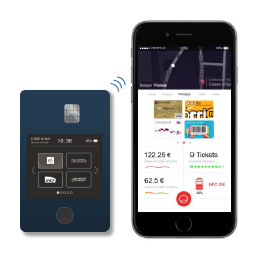
\includegraphics[scale=0.5]{img/carte.png}
			\caption{\label{Carte} Concept de la carte universelle connectée.}			
\end{figure}

Le travail qui nous a été demandé concernait surtout l'aspect bancaire, et plus particulièrement le transport d'informations contextuelles au sein d'une transaction EMV. C'est pourquoi la première partie de notre travail a consisté à étudier la spécification EMV "Payment Tokenisation Specification", de manière à nous familiariser avec la Tokenisation.


\section{Introduction à la Tokenisation}
\subsection{Définition d'un Token}
Dans le cadre d'une transaction, un Token est une donnée "jetable", aussi appelée jeton de paiement, permettant de remplacer les données bancaires telles que le PAN (Personal Account Number). Ainsi, le processus de Tokenisation consiste à générer un Token à partir du PAN et de sa date d'expiration [Figure \ref{Tokenisation}].

\begin{figure}[!h]
    \centering
			\includegraphics[scale=0.75]{img/tokeniser2.png}
			\caption{\label{Tokenisation} Principe de la Tokenisation.}			
\end{figure}

Inversement, le processus de Detokenisation permet de récupérer le PAN et sa date d'expiration à partir du Token [Figure \ref{Detokenisation}]. 

\begin{figure}[!h]
    \centering
			\includegraphics[scale=0.75]{img/detokeniser.png}
			\caption{\label{Detokenisation} Principe de la Detokenisation.}			
\end{figure}

\subsection{Pourquoi les Token?}
\noindent
\underline{Dans le cadre des transactions EMV}:\\

\noindent
L'utilité des Tokens réside dans le fait qu'ils permettent d'assurer l'intégrité et la confidentialité du PAN lors d'une transaction EMV. En effet, en cas d'interception, le PAN a peu de chance d'être récupéré ce qui limite les risques. Cela permet aux banques émetteurs de réduire la fraude et aux commerçants de ne pas avoir à stocker les informations clients dans leur système d'information.\\

\noindent
De ce fait, les Tokens sont notamment utilisés lors des paiements NFC (Near Field Communication), lors de l'utilisation d'une wallet (i.e. Apple Pay) ou dans le domaine du e-Commerce.\\

\noindent
\underline{Dans le cadre du projet}:\\

\noindent
En plus d'être un élément de sécurité, l'utilisation des Tokens nous permet de transporter de l'information supplémentaire lors des transactions.


\newpage
\section{Planning}
\begin{figure}[!ht]
    \centering
			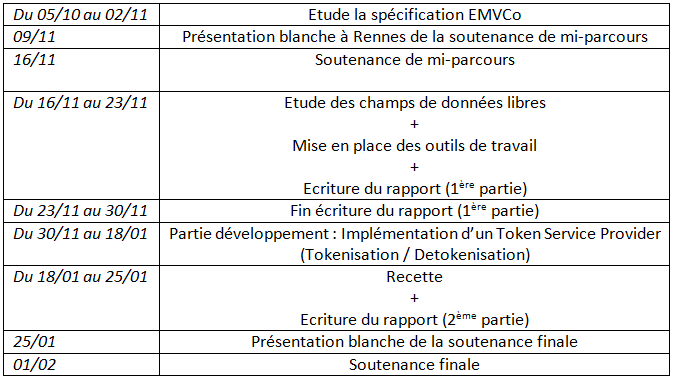
\includegraphics[scale=0.9]{img/planningFinal.png}
			\caption{\label{Planning} Planning final du projet.}			
\end{figure}



\chapter{Etude de la spécification EMVCo "Payment Tokenisation Specification", 2014}
Dans ce chapitre, nous allons revenir sur notre étude de la spécification pour détailler les différentes phases d'une transaction avec Token de façon claire. Dans un premier temps, nous introduirons deux nouveaux acteurs qui n'interviennent pas dans une transaction EMV classique, mais seulement dans une transaction avec Token. Ensuite, nous présenterons les différents éléments de données avant de nous intéresser de plus près à une transaction EMV avec Token, à travers quatre cas d'usage bien précis.\\

\noindent
Ci-dessous se trouve le schéma global d'une transaction EMV avec Token [Figure \ref{TransactionScheme}]. Dans les parties 2.3, 2.4 et 2.5, nous allons découper ce schéma pour le détailler plus amplement.

\begin{figure}[!ht]
    \centering
			\includegraphics[scale=0.6]{img/TransactionSchemeTokenPAN.png}
			\caption{\label{TransactionScheme} Schéma global d'une transaction EMV avec Token.}			
\end{figure}

 
\section{Token Service Provider et Token Requestor}
\subsection{Token Service Provider}
Le Token Service Provider a pour rôle de fournir les Tokens et de gérer leur cycle de vie. Pour cela, il se doit également d'implémenter toutes les interfaces liées aux services du Token et de garantir la sécurité du Token ainsi que l'association PAN / Token.\\
Lors d'une transaction, le Token Service Provider peut être n'importe quel acteur, c'est-à-dire, la banque émetteur, la banque acquéreur, le commerçant, le réseau de paiement ou encore une tierce partie.

\subsection{Token Requestor}
Le Token Requestor est, quant à lui, responsable des demandes de génération de Token et de changement d'état du Token, notamment en cas de perte ou de vol de celui-ci. Toutefois, avant de pouvoir faire une demande de génération de Token, le Token Requestor doit impérativement s'être au préalable enregistré auprès d'un ou plusieurs Token Service Provider.\\
Lors d'une transaction, le token Requestor peut être la banque émetteur, la banque acquéreur, le commerçant ou bien une tierce partie comme par exemple un gestionnaire de wallet. Cependant, contrairement au Token Service Provider, le Token Requestor ne sera en aucun cas le réseau de paiement.


\section{Les Data elements}
Les Data elements ou éléments de données qui sont utilisés dans une transaction initiée avec un Token, sont présentés dans le schéma ci-dessous [Figure \ref{DataElements}]. Ils peuvent être obligatoires, conditionnels ou optionnels suivant le message auquel ils appartiennent et suivant l'API utilisée. Tous les réseaux de paiement doivent supporter ces éléments de données lors d'une transaction, pour assurer l'interopérabilité entre les réseaux de paiement.\\

\noindent
Dans un soucis de clarté du schéma, nous avons seulement représenté les éléments de données qui transitent entre deux entités.\\
Pour plus de précisions sur ces éléments de données, consulter la partie 4 de la spécification, "Payment Token Specification Data Elements", à l'adresse suivante: \textit{https://www.emvco.com/specifications.aspx?id=263}.

\begin{figure}[!ht]
    \centering
			\includegraphics[scale=0.5]{img/data_elements.png}
			\caption{\label{DataElements} Eléments de données fournis par une entité à une autre pour une transaction avec Token.}			
\end{figure}

Le Token Vault est un endroit, appartenant au Token Service Provider, dans lequel sont stockés l'association PAN/Token, le Token Requestor ID ainsi que la date d'expiration du Token.


\section{Demande et émission de Token}
Lors d'une transaction EMV, lorsque le PAN n'est pas déjà lié à un Token valide et qu'un Token est requis, le Token Requestor envoie une demande de génération de Token au Token Service Provider. Cette requête contient donc le PAN et sa date d'expiration, ainsi que le Token Requestor ID. Ensuite, le Token service Provider va se charger d'envoyer une demande d'identification et vérification à la banque émetteur, pour déterminer le Token Assurance Level et le Token Assurance Data. Une fois cette étape validée, le Token Service Provider génère le Token qu'il transmet au Token Requestor, en plus de la date d'expiration du Token, du Token Assurance Level et du Token Assurance Data.\\

\noindent
Le schéma suivant résume la demande et l'émission d'un Token [Figure \ref{DemandeEmissionToken}].

\begin{figure}[!ht]
    \centering
			\includegraphics[scale=0.6]{img/demandeETemissionToken.png}
			\caption{\label{DemandeEmissionToken} Demande et émission d'un Token.}			
\end{figure}

Dans les deux sous-parties qui suivent, nous présenterons davantage les méthodes d'identification et vérification, et les interfaces qui doivent être implémentées par le Token Service Provider.

\subsection{Les méthodes d'Identification et Vérification}

\subsubsection{Généralités}
Les méthodes d'Identification et de Vérification (ID \& V) fournissent la confiance nécessaire à une association entre le PAN et un Token par des vérification diverses sur le porteur ou sur le compte du porteur. Tout cela pour fournir un cadre fiable de paiment par Token. \\
Le Token Assurance Level est une donnée importante pour les paiements utilisant des tokens. Ce Token Assurance Level est dérivé de la méthode d'ID \& V utilisée.
Deux Data Elements sont utilisés pour fournir des informations sur le Token Assurance Level et les méthodes d'ID \& V utilisées.\\
Ce sont les champs : 
\begin{itemize}
	\item Token Assurance Level
	\item Token Assurance Data\\
\end{itemize}

Le Token Service Provider \textbf{DOIT} mettre en place les interfaces nécessaires pour fournir ces deux Data Elements.
Le Token Assurance Level est un nombre compris entre 00 et 99 en fonction du niveau des vérifications effectuées. Le Token Service Provider \textbf{DOIT} également associer le bon Token Assurance Level en fonction des vérifications effectuées.

\subsubsection{Les différentes méthodes}
Il n'y a pas vraiment de méthodes d'ID \& V imposées, mais le Token Service Provider \textbf{DOIT} implémenter une ou plusieurs méthodes d'ID \& V et \textbf{DOIT} assurer que la méthode requise est employé lors de la génération d'un Token. Certaines étapes de ces vérification peuvent être faites par le Token Service Provider, le Token Requestor ou par une tierce partie. Mais dans le cas où les vérifications ne sont pas effectuées par le Token Service Provider, l'entité ayant effectuée une étape de la vérification \textbf{DOIT} fournir des preuves vérifiables du résultat des vérifications.\\
Les vérifications mentionnées dans la spécification sont les suivantes:\\
\begin{itemize}
	\item Pas de vérification
	\item Vérification du compte (Autorisation à 0 ou autres méthodes.)
	\item Calcul d'un score de risque en utilisant les données du Token Service Provider.
	\item Calcul d'un score de risque en utilisant en plus des données du réseau de paiement.
	\item Vérification du porteur (3DSecure par exemple)
\end{itemize}


\subsection{Les interfaces: Token Service Provider APIs}
\subsubsection{Généralités}
Le Token Service provider \textbf{DOIT} mettre en place une manière sécurisée d'intéragir avec les entités utilisant ses services, à travers par exemple, un Web Service, la norme ISO 8583 ou encore des batches.\\
Le Token Service Provider \textbf{PEUT} implémenter les différentes interfaces et les rendre accessibles aux entités voulant utiliser ses services. Les différentes catégories d'interface sont:
\begin{itemize}
	\item Token Request et Token Assurance
	\item Token Assurance (ID \& V)
	\item De-Tokenisation
	\item Token Routing
	\item Token Lifecycle Management
\end{itemize}
\noindent
Le Token Service Provider \textbf{DOIT} mettre en place au moins une interface par catégorie.

\subsubsection{Token Request et Token Assurance}
Le Token Service Provider \textbf{DOIT} fournir une méthode permettant, à un Token Requestor qui s'est enregistré auprès de lui, de demander l'émission d'un Token.
Le Token Service Provider \textbf{DOIT} aussi mettre en place les contrôles nécessaires pour générer le Token. De plus, il peut effectuer des opérations d'assurance supplémentaires. Dans ce cas, il \textbf{PEUT} indiquer dans sa réponse les mécanismes de vérifications utilisés. 

\subsubsection{Token Assurance}
Toutes ces méthodes sont utilisées si, après l'émission d'un Token, le Token Requestor souhaite faire une mise-à-jour du niveau d'assurance.

\subsubsection{De-Tokenisation}
Le Token Service Provider \textbf{DOIT} mettre en place les contrôles appropriés pour authentifier l'entité qui fait la demande de dé-tokenisation.

\subsubsection{De-Tokenisation avec vérification}
Le Token Service Provider doit, en plus de la dé-tokenisation classique, effectuer des vérifications complémentaires pour s'assurer que le Token est bien utilisé dans un des domaines pour lesquels il a été généré. L'ensemble de ces domaines s'appelle le Token Domain Restriction Controls. 

\subsubsection{Token Lifecycle Management}
Le Token Service Provider \textbf{DOIT} mettre en place des moyens de gérer le cycle de vie d'un Token émis. Ces interfaces peuvent êtres utilisées par de nombreuses entités telles que le réseau de paiement, le Token Requestor, la banque émettrice, etc.\\

\noindent
L'implémentation de TOUTES ces interfaces est laissée à la discretion du Token Service Provider.


\section{Transaction EMV avec Token}
Dans cette section, nous allons d'abord présenter l'interaction client-commerçant de manière à introduire les différents cas d'usage, impliquant un Token, utilisés dans la spécification. Dans un second temps, nous verrons comment se poursuit la transaction avec le Token, depuis le commerçant vers les autres acteurs de la transaction.

\subsection{Côté client - commerçant}
Dans la spécification, l'interaction client - commerçant, lors d'une transaction EMV avec Token, est présentée à travers les paiements NFC mobile, par QR code, par wallet et via les sites de e-Commerce.\\

\noindent
Ce dernier cas est d'ailleurs un peu particulier puisque, lorsque le client fait des achats sur le site d'un commerçant pour la première fois, celui-ci va lui demander de lui envoyer le PAN [Figure \ref{CardOnFile}]. En général, le client doit remplir un formulaire avec les données inscrites sur sa carte. Le PAN ne sera pas stocké par le commerçant mais celui-ci va directement contacter le Token Requestor pour qu'il fasse une demande de génération de Token. Par la suite, c'est le Token qui sera stocké par le commerçant. C'est ce qu'on appelle le Card-on-File. Ainsi, le client est en quelque sorte enregistré auprès du commerçant, et lorsqu'il fera d'autres achats sur ce site, le commerçant utilisera le Token lié au PAN du client, qu'il aura conservé dans un fichier. Ici, c'est donc côté commerçant qu'est stocké le Token.\\

\begin{figure}[!ht]
    \centering
			\includegraphics[scale=0.6]{img/cof.png}
			\caption{\label{CardOnFile} Interaction client-commerçant pour le cas d'usage Card-on-file.}			
\end{figure}

Pour les trois autres cas d'usage, le Token est conservé côté client, c'est-à-dire, stocké dans l'appareil du client, qui est son téléphone mobile dans la plupart des cas. En effet, lors d'une transaction, c'est le client qui envoie au commerçant le Token, sa date d'expiration, le Token cryptogram et éventuellement le Token Requestor ID [Figure \ref{ClientCommercant}].\\
A noter également que, dans le cas du QR code, le client transmet aussi les données du QR code au commerçant. Dans le cas du NFC mobile, il peut y avoir des échanges de données avec un cloud au préalable.

\begin{figure}[!ht]
    \centering
			\includegraphics[scale=0.6]{img/interaction_client-commercant2.png}
			\caption{\label{ClientCommercant} Interaction client-commerçant pour les cas d'usage: NFC mobile, Wallet, QR Code.}			
\end{figure}

\subsection{Côté commerçant - autres acteurs de la transaction}
Une fois la transaction engagée entre le client et le commerçant, ce dernier envoie une demande d'autorisation à sa banque acquéreur et lui transmet les données que le client lui a envoyé ainsi que le Point Of Sell Entry Mode ou mode d'acceptation [Figure \ref{CommercantAutresActeurs}]. Dans le cas du e-Commerce, l'identifiant du commerçant est également transmis à la banque acquéreur.\\
Ensuite, celle-ci va rediriger toutes ces données vers le réseau de paiement, qui va alors contacter le Token Service Provider pour que celui-ci fasse l'association entre le Token et le PAN correspondant. Le Token Service Provider renvoie donc le PAN au réseau de paiement, mais aussi le Token Assurance Data et le Token Assurance Level. C'est la phase de detokenisation. Ainsi, le réseau de paiement va envoyer les données qu'il a reçu de la banque acquéreur et du Token Service Provider à la banque émetteur, c'est-à-dire, le couple PAN/Token et les données correspondantes. La banque émetteur reçoit donc la demande d'autorisation et peut ou non la valider.\\
Enfin, le résultat de la demande d'autorisation et le PAN sont retransmis au réseau de paiement qui va remplacer le PAN par le Token correspondant, avant de faire recirculer ces données vers la banque acquéreur, qui va les transmettre au commerçant.\\

\noindent
Le schéma ci-dessous résume le déroulement d'une transaction EMV avec Token, à partir du commerçant.

\begin{figure}[!ht]
    \centering
			\includegraphics[scale=0.6]{img/interaction_commercant-autres.png}
			\caption{\label{CommercantAutresActeurs} Interaction commerçant-autres acteurs de la transaction.}			
\end{figure}


\section{Acquisition, compensation, gestion des impayés}
Dans cette partie, nous allons présenter les processus d'acquisition, de compensation et de gestion des impayés, qui se déroulent pendant et après la télécollecte.\\

\noindent
Dans le cadre du projet, nous ne nous intéresserons pas à ces trois phases, mais il est nécessaire de les détailler ici puisqu'elles sont présentées dans la spécification.

\subsection{Acquisition et compensation}
Lors de la phase d'acquisition/compensation, le commerçant envoie d'abord un fichier d'acquisition à sa banque acquéreur. Ce fichier contient le Token, sa date d'expiration, le Token Assurance Level et éventuellement le Token Requestor ID. Ensuite, la banque acquéreur vérifie les éléments de données contenus dans ce fichier et y ajoute le mode d'acceptation pour constituer un fichier de compensation qu'elle va envoyer au réseau de paiement. Tout comme pour la transaction, celui-ci va demander au Token Service Provider de faire le mapping entre le Token et le PAN pour pouvoir ensuite transmettre le fichier de compensation complété à la banque émetteur, qui devra valider ou non la compensation et renvoyer sa réponse au réseau de paiement.\\

\newpage
\noindent
Le schéma ci-dessous détaille les champs de données qui transitent lors des phases d'acquisition puis de compensation [Figure \ref{CaptureClearing}].

\begin{figure}[!ht]
    \centering
			\includegraphics[scale=0.6]{img/CaptureClearing.png}
			\caption{\label{CaptureClearing} Acquisition et compensation d'une transaction réalisée avec un Token.}			
\end{figure}

\subsection{Gestion des impayés}
En cas de transaction impayée, la banque émetteur fournit le PAN, le Token et éventuellement le Token Requestor ID au réseau de paiement. Celui-ci envoie alors le PAN au Token Service Provider qui va effectuer un certain nombre de vérifications sur le Token et sur le mapping PAN/Token, comme par exemple, s'assurer de la validité du Token ou de l'association avec le PAN. Ensuite, le réseau de paiement transmet la demande de gestion de l'impayé, contenant le Token, à la banque acquéreur qui enquêtera pour savoir si elle accepte ou non cette requête.\\

\noindent
Le schéma qui suit représente la phase de gestion des impayés vue précédement [Figure \ref{Impayes}].

\begin{figure}[!ht]
    \centering
			\includegraphics[scale=0.6]{img/Chargeback.png}
			\caption{\label{Impayes} Phase de gestion des impayés effectuée après une transaction avec Token.}			
\end{figure}



\chapter{Implémentation d'un Token Service Provider}
Grâce à la lecture de la spécification présentée au chapitre précédent, nous avons pu implémenter un Token Service Provider pour répondre aux besoins du projet One Wave. Dans la suite de ce chapitre, nous allons présenter l'architecture de notre solution et expliquer nos choix d'implémentation.

\section{Architecture du projet}
Tout est implémenté en Java, avec pour contrainte de pouvoir être embarqué sur une puce par la suite.\\
Le diagramme de classe ci-dessous présente l'architecture générale du projet, découpé en quatre modules [Figure \ref{Architecture}].

\begin{figure}[!ht]
    \centering
			\includegraphics[scale=0.5]{img/ClassDiagramm.png}
			\caption{\label{Architecture} Diagramme de classe de l'architecture du projet.}			
\end{figure}

\noindent
Nous allons maintenant expliquer plus en détails cette architecture et la façon dont nous l'avons implémentée.

\newpage
\subsection{Les différents modules}
\noindent
\textbf{Tokenizer}: Génère le Token à partir du PAN, sur demande d'un Token Requestor.\\

\noindent
Pour cela, nous avons créé une interface \textit{Tokenizer} qui est implémentée par les classes \textit{TokenizerRSA} et \textit{TokenizerAES}. Nous pouvons donc avoir un Tokenizer pour chaque algorithme de chiffrement. Par ailleurs, la tokenisation avec AES se fait en mode "PKCS5Padding" alors que celle avec RSA se fait en mode "OAEPWithSHA-256AndMGF1Padding". Nous avons utilisé ici la classe \textit{Cipher} de la librairie \textit{Javax}, implémentée à cet effet. Nous avons aussi créé une classe \textit{InputReader} qui permet de lire le message d'entrée de la Tokenisation et qui récupère un à un les différents champs de données. Une classe \textit{TokenizerServer} charge les clés, ouvre une socket serveur et lance un thread qui a pour routine une instance de la classe \textit{TokenizerJob}. C'est cette dernière classe qui s'occupe de Tokeniser.\\

\noindent
Toutes les relations entre ces classes sont représentées dans le diagramme de classe ci-dessous [Figure \ref{ArchitectureTokenizer}].

\begin{figure}[!ht]
    \centering
			\includegraphics[scale=0.7]{img/TokenizerDiagramm.png}
			\caption{\label{ArchitectureTokenizer} Diagramme de classe du module Tokenizer.}			
\end{figure}

\noindent
\textbf{Detokenizer}: Retrouve le PAN à partir du Token sur demande d'une autorité authentifiée telle que le réseau de paiement.\\

\noindent
Comme pour le module précédent, nous avons créé une interface \textit{Detokenizer} qui est implémentée par les classes \textit{DetokenizerRSA} et \textit{DetokenizerAES}. Nous pouvons donc avoir un Detokenizer pour chaque algorithme de chiffrement. Par ailleurs, la detokenisation avec AES se fait en mode "PKCS5Padding", et celle avec RSA se fait en mode "OAEPWithSHA-256AndMGF1Padding", à l'image de la Tokenisation. Nous avons utilisé là aussi la classe \textit{Cipher} de la librairie \textit{Javax}. La classe \textit{InputReader} permet cette fois de lire le message d'entrée de la Detokenisation et de récupérer un à un les différents champs de données. La classe \textit{DetokenizerServer} charge les clés, ouvre une socket serveur et lance un thread qui a pour routine une instance de la classe \textit{DetokenizerJob}. Cette dernière classe s'occupe de Detokeniser.\\

\noindent
Toutes les relations entre ces classes sont représentées dans le diagramme de classe ci-après [Figure \ref{ArchitectureDetokenizer}].

\begin{figure}[!ht]
    \centering
			\includegraphics[scale=0.7]{img/DetokenizerDiagramm.png}
			\caption{\label{ArchitectureDetokenizer} Diagramme de classe du module Detokenizer.}			
\end{figure}

\noindent
\textbf{Token Service Provider}: Agrège les deux modules précédents et fournit les API correspondantes.\\

\noindent
Dans ce module, une interface \textit{TokenServiceProvider} est implémentée par une classe abstraite \textit{AbstractTokenServiceProvider} qui nous permet de factoriser la suite du code et de définir le comportement par défaut des classes qui vont en hériter. Ces classes sont, logiquement, \textit{TokenServiceProviderAES} et \textit{TokenServiceProviderRSA}. Nous pouvons donc, ici aussi, avoir un Token Service Provider pour chaque algorithme de chiffrement. Une classe \textit{TokenServiceProviderServer} lance les serveurs de Tokenisation et de detokenisation.\\

\noindent
Ce module est représenté par le schéma de la figure [Figure \ref{ArchitectureTSP}].\\

\begin{figure}[!ht]
    \centering
			\includegraphics[scale=0.7]{img/TokenServiceProvider.png}
			\caption{\label{ArchitectureTSP} Diagramme de classe du module TokenServiceProvider.}			
\end{figure}

\noindent
\textbf{Token Requestor}: Implémenté pour la démonstration, il interroge le Tokenizer et/ou le Detokenizer.\\

\noindent
Une classe \textit{TokenRequester} créé et lance trois threads instanciés grâce à une classe \textit{TokenRequesterJob}. Ces trois threads correspondent à trois clients qui enverront successivement des demandes de Tokenisation et de Detokenisation, et qui s'assureront que le PAN obtenu à la fin correspond bien au PAN généré aléatoirement au début. La classe \textit{TokenRequesterJob} redéfinie la méthode \textit{run()} pour les threads.\\

\noindent
Ces deux classes sont représentées sur le schéma de la figure [Figure \ref{ArchitectureTR}].

\begin{figure}[!ht]
    \centering
			\includegraphics[scale=0.7]{img/TokenRequester.png}
			\caption{\label{ArchitectureTR} Diagramme de classe du module TokenRequester.}			
\end{figure}

\newpage
\subsection{La programmation côté serveur}
Pour fonctionner, ces modules ont besoin d'interagir avec l'extérieur (demande de Tokenisation au Tokenizer, etc.). Voilà pourquoi nous avons crée un serveur pour la Tokenisation et pour la Detokenisation. Nous avons aussi utilisé le Token Requestor comme client pour pouvoir envoyer des requêtes à ces serveurs.\\
Tous les serveurs sont pour le moment mono-thread. Par la suite, la Tokenisation ne se fera surement pas par un serveur car le module sera embarqué sur une carte à puce. Pour la Detokenisation, il serait possible d'utiliser le multi-threading, mais cela n'était pas nécessaire pour les besoins de la démonstration.\\

\noindent
Le listing ci-dessous donne le code de la méthode \textit{main()} de la classe \textit{TokenizerServer}, et montre comment la Tokenisation est lancée côté serveur. Le principe est le même pour les trois autres modules.\\

\begin{lstlisting}
public static void main(String[] args) throws IOException {
        if (args.length != 0) {
            loadKey(args[0]);
        } else {
            loadKey();
        }
        ServerSocket serverSocket = new ServerSocket(2009);
        Thread tokenizer = new Thread(new TokenizeJob(serverSocket, publicKey));
        tokenizer.start();
}
\end{lstlisting}

\subsubsection{AES et RSA}
Etant donné qu' il n'y a pas de communication directe entre le Tokenizer et le Detokenizer (pas de Token Vault), il nous a fallu utiliser la cryptographie pour chiffrer les échanges de PAN et de Token entre ces deux entités. Nous avons d'abord utilisé un chiffrement AES pour des questions de performances et de taille des données échangées. Le problème avec ce système cryptographique, c'est qu'il nécessite une clé partagée, et ce pour chacun des Tokenizers. Nous nous sommes donc orientés vers le chiffrement RSA qui permet au Detokenizer de n'avoir qu'une seule clé privée, permettant de déchiffrer n'importe quel Token chiffré avec sa clé publique et donc de retrouver le PAN correspondant.\\
Par le biais du Token Service Provider, il est possible d'étendre notre modélisation à d'autres systèmes de chiffrement, puisque ce module comporte une interface qui implémente un Tokenizer et un Detokenizer pour chacun de ces systèmes.\\

\noindent
Nous avons testé les performances de notre implémentation avec le profiler de la JVM. Celui-ci a retourné un temps d'exécution de 34ms pour la démonstration en utilisant RSA. Nous n'avons pas testé la démonstration avec AES puisque ce système de chiffrement ne sera surement pas utilisé par la suite, du fait des inconvénients liés aux clés.

\subsubsection{La gestion des données}
Les seules données que nous stockons sont le couple clé publique / clé privée utilisé pour la Tokenisation et la Detokenisation. Ces clés sont stockées respectivement dans les fichiers \textit{public.key} et \textit{private.key} que nous avons choisi de placer dans les ressources du projet Maeven. Il est possible de mettre ces deux fichiers ailleurs, mais il faut dans ce cas changer la valeur de la variable "path" passée en paramètre des méthodes de la classe \textit{KeyUtils} (voir plus bas \textbf{Les classes utilitaires}).


\subsection{Les types de données}
Nous avons utilisé des tableaux d'octets pour représenter les données définies dans la spécification car il s'agit du format standard pour échanger des données. Nous avions commencé par utiliser des chaînes de caractères mais cette modélisation ne permettait pas de manipuler les données membres à nos souhaits.\\
De plus, les tableaux d'octets sont des types de données utilisés en Javacard, contrairement aux chaînes de caractères, ce qui convient à la consigne qui nous a été donnée.

\subsection{Les classes utilitaires}
Nous avons jugé bon de créer un module \textit{Utils} dans lequel se trouvent un certain nombre de classes utilitaires. Celles-ci permettent d'éviter la duplication de code et de simplifier le traitement des données.\\

\noindent
\textbf{BytesUtils}: Tous les champs de données sont concaténés dans un tableau d'octets pour constituer le message d'entrée pour la Tokenisation. Cette classe effectue un padding sur un tableau d'octets contenant le PAN. Ce padding est fait sur les premières cases du tableau pour ne pas modifier la valeur des données déjà présentes dans le tableau. Ainsi, le champ de données réservé au PAN est toujours de la même taille, ce qui simplifie le traitement des données suivantes. En revanche, ce traitement ne tient pas compte des aspects sécuritaires, c'est-à-dire qu'il est possible que cela introduise d'éventuelles failles de sécurité.\\

\noindent
\textbf{KeyUtils}: Effectue de petits traitements sur les clés.
\begin{itemize}
	\item Sauvegarde d'une clé publique dans le fichier \textit{public.key} dans le dossier choisi. La clé est encodée avec le certificat X509.
	\item Sauvegarde d'une clé privée dans le fichier \textit{private.key} dans le dossier choisi. La clé est encodée avec le standard PKCS8.
	\item Sauvegarde d'une paire de clés publique/privée grâce aux deux méthodes utilisées pour les traitements ci-dessus.
	\item Chargement d'une clé publique dans le fichier \textit{public.key}.
	\item Chargement d'une clé privée dans le fichier \textit{private.key}.
	\item Chargement d'une paire de clés publique/privée grâce aux deux méthodes utilisées pour les traitements ci-dessus.
\end{itemize}

~\\
\noindent
\textbf{MessageUtils}: Construit le message d'entrée pour la Tokenisation en concaténant les champs de données requis dans un tableau d'octets, à l'aide de la classe \textit{BytesUtils}.\\

\noindent
\textbf{SocketUtils}: 
\begin{itemize}
	\item Lis le contenu du flux entrant d'une socket (InputStream) qui est ensuite récupéré dans un tableau de 2048 bits.
	\item Ecris le contenu d'un tableau de 2048 bits dans le flux sortant d'une socket (OutputStream).
\end{itemize}

~\\
\noindent
\textbf{TransactionMock}: Effectue les transformations nécessaires sur le message de sortie de la Tokenisation pour que les champs de données correspondent à ceux demandés, par la spécification EMVCo, pour le message d'entrée de la Detokenisation.

\subsection{Le fonctionnement global du projet}
Pour lancer les serveurs de Tokenisation et de Detokenisation ainsi que les requêtes client du Token Requestor nous passons par une API. Les commandes suivantes permettent respectivement de lancer le serveur de Tokenisation, le serveur de Detokenisation et les clients:

\begin{center}
	\begin{lstlisting}
		java -jar tokenizer.jar .
		java -jar detokenizer.jar .
		java -jar tokenrequester.jar
	\end{lstlisting}
\end{center}

\noindent
Le programme tourne alors indéfiniment, c'est-à-dire que les trois clients envoient successivement des demandes de Tokenisation et de Detokenisation jusqu'à ce qu'on arrête l'exécution manuellement. A chaque demande de Tokenisation envoyée par l'un des clients, un message d'entrée (pour la Tokenisation) est généré grâce à la classe \textit{MessageUtils}. Ce message est alors transmis au Tokenizer qui génère un Token et retourne un message de sortie conforme à ce qui est demandé dans la spécification. La classe \textit{TransactionMock} transforme ensuite ce message de sortie pour constituer le message d'entrée pour la Detokenisation. Le Detokenizer retrouve le PAN et genère à son tour un message de sortie. Là encore ce message respecte la spécification. Tous les champs de données présents dans les différents messages sont d'abord récupérés individuellement dans des tableaux d'octets puis concaténés dans un nouveau tableau d'octets grâce à la classe \textit{BytesUtils} chargée de faire les paddings nécessaires.\\

\noindent 
Pour compiler l'ensemble du projet, il faut utiliser la commande suivante:

\begin{center}
	\begin{lstlisting}
		maeven clean package
	\end{lstlisting}
\end{center}

\noindent
Cela génère tous les fichier .jar de l'application et copie les fichiers de clé (public.key et private.key) dans le dossier \textit{out} à la racine du projet.


\section{Contrôle de qualité}
Nous avons souhaité tester notre code source à chaque nouvelle implémentation, de manière à toujours avoir un résultat fonctionnel.  

\subsection{Les tests unitaires}
Dans un premier temps, des tests unitaires ont été implémentés sur chacune des classes des modules Tokenizer, Detokenizer et Token Service Provider (sauf sur les classes serveur du Tokenizer et du Detokenizer). Nous avons essayé de tester un maximum de lignes de code bien qu'il soit difficile de tester les blocs try/catch. Pour ces trois modules, le taux de coverage est donc très élevé.\\
Aucun test unitaire n'a été crée ni pour les classes utilitaires, puisqu'elles sont utilisées dans les classes de tests, ni sur le module Token Requestor car il a été implémenté seulement pour la démonstration et parce qu'il ne fait pas partie du rendu final.\\
A ce jour, 19 tests unitaires existent et ils sont tous au vert.

\subsection{Les tests d'intégration}
Le Token Service Provider a servi à réaliser les tests d'intégration et à nous assurer du bon interfaçage entre les modules Tokenizer et Detokenizer.\\
En résumé, nous avons crée des PAN que nous avons ensuite donnés au Token Service Provider pour que celui-ci demande au Tokenizer de tokeniser puis au Detokenizer de detokeniser, une fois les Tokens correspondants générés. A la fin, une comparaison est faite entre le PAN retrouvé après Detokenisation et le PAN de départ pour confirmer le bon fonctionnement des modules concernés. 

\newpage
\section{Démonstration finale}
Les trois captures d'écran ci-dessous montrent les requêtes envoyées par le Token Requestor qui arrivent aux serveurs de Tokenisation et de Detokenisation, avec réception respectivement du PAN et du Token, et renvoi de ceux-ci au Token Requestor. Toutes ces requêtes sont envoyées à intervalles de temps aléatoires, au serveur qui leur correspond, pour mieux simuler une situation réelle. 

\begin{figure}[!ht]
    \centering
			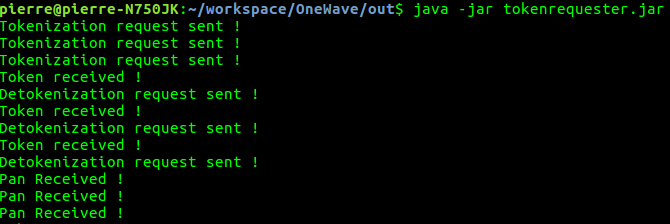
\includegraphics[scale=0.47]{img/client_tokenRequestor.png}
			\caption{\label{Trello} Envoi des requêtes de Tokenisation/Detokenisation et réception des PANs/Tokens correspondants par le Token Requestor.}			
\end{figure}

\begin{figure}[!ht]
    \centering
			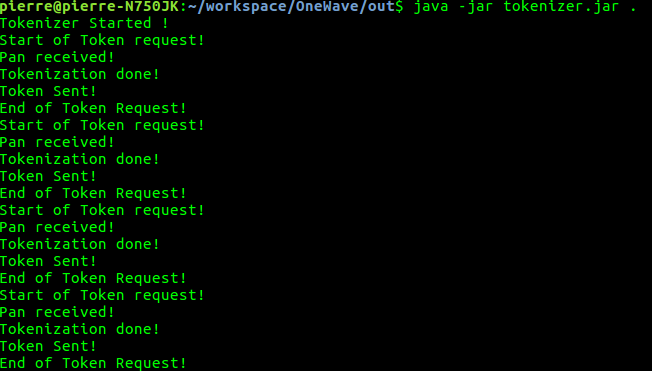
\includegraphics[scale=0.47]{img/serveur_tokenizer.png}
			\caption{\label{Trello} Réception des PANs, Tokenisation et envoi des Tokens correspondants par le serveur de Tokenisation.}			
\end{figure}

\begin{figure}[!ht]
    \centering
			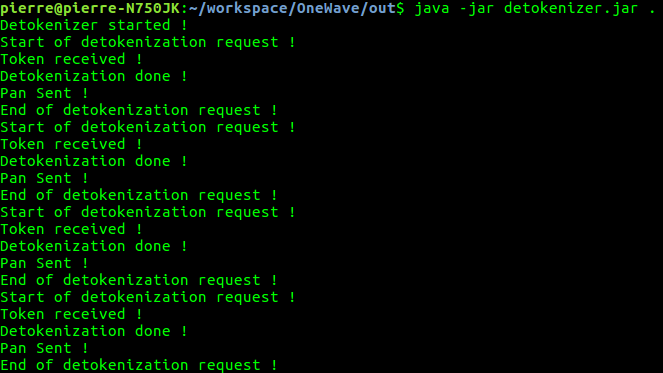
\includegraphics[scale=0.47]{img/serveur_detokenizer.png}
			\caption{\label{Trello} Réception des Tokens, Detokenisation et envoi des PANs correspondants par le serveur de Detokenisation.}			
\end{figure}


\chapter{Gestion de projet}
L'aboutissement de ce projet repose en partie sur notre organisation et sur le choix de nos outils de travail. 

\section{Organisation de l'équipe projet}
Pendant la phase d'étude de la spécification, nous avons fait une lecture chacun de notre côté puis nous avons travaillé ensemble sur le résumé présenté dans le chapitre II.\\
Au moment de commencer l'implémentation du Token Service Provider, nous nous sommes d'abord mis d'accord avec notre tuteur entreprise sur l'architecture à implémenter, puis nous nous sommes répartis les différents modules:\\

\begin{itemize}
	\item Eglantine: Detokenizer.
	\item Pierre: Tokenizer, Token Service Provider.
\end{itemize}

~\\
\noindent
Nous avons ensuite travaillé ensemble sur le Token Requestor et sur la programmation côté serveur.

\section{Les outils de gestion de projet}
Pour l'organisation des tâches au sein du groupe nous avons utilisé \textbf{Trello} pendant la phase d'étude de la spécification. Ci-dessous se trouve une capture d'écran prise pendant cette période et montrant comment nous nous sommes organisés [Figure \ref{Trello}]. 

\begin{figure}[!ht]
    \centering
			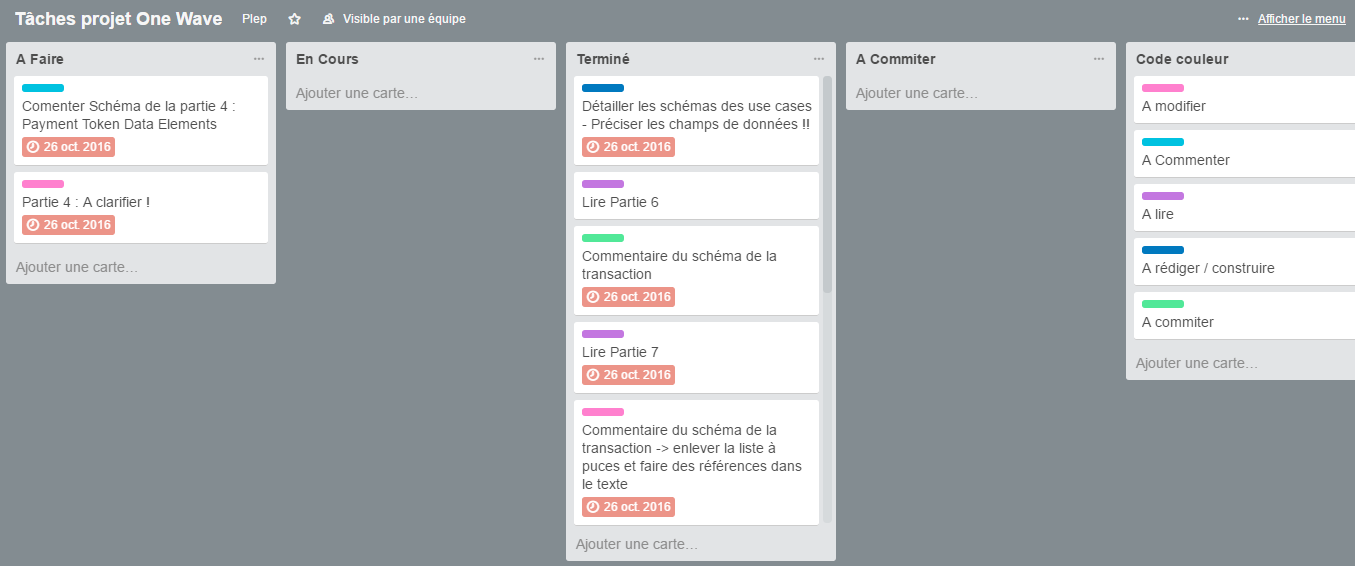
\includegraphics[scale=0.46]{img/trello.PNG}
			\caption{\label{Trello} L'organisation des tâches avec Trello.}			
\end{figure}

\newpage
\noindent
Nous avons aussi utilisé \textbf{draw.io} pour construire tous les schémas présents dans le rapport et dans les présentations orales.

\begin{figure}[!ht]
    \centering
			
\includegraphics[scale=0.2]{img/draw.png}
			\caption{\label{Draw} draw.io.}			
\end{figure}

\noindent
Pour toute la partie implémentation du Token Service Provider nous nous sommes servis de l'IDE Java \textbf{IntelliJ}, développé par \textbf{JetBrains}, dont nous avons pu obtenir une licence gratuitement grâce à notre statut d'étudiant.

\begin{figure}[!h]
		\centering
    \begin{subfigure}[b]{0.2\textwidth}
        
\includegraphics[width=\textwidth]{img/intellij.jpg}
        \caption{IntelliJ.}
    \end{subfigure}
    \begin{subfigure}[b]{0.2\textwidth}
        
\includegraphics[width=\textwidth]{img/jetbrains.png}
        \caption{JetBrains.}
    \end{subfigure}
\end{figure}

\noindent
Cet IDE intègre un menu dédié à la gestion des VCS (Version Control System), ce qui nous a permis d'interagir facilement avec le dépôt Git que nous avions en commun avec notre tuteur entreprise. De cette manière, nous avons pu lui mettre tout le code source à disposition pour qu'il ait directement accès au prototype.


\section{Rencontres avec les tuteurs et le client}
Nous avons fait le point avec notre client/tuteur, Léonard Dallot, par Skype toutes les semaines, pour lui présenter les dernières progressions et programmer les tâches à réaliser pour la semaine suivante. La première séance a été consacrée à l'établissement d'un planning de travail pour toute la période de réalisation du projet. Ce planning a d'ailleurs été tenu de bout en bout. Nous avons également eu l'occasion de nous déplacer à Rennes les semaines précédent les soutenances finale et de mi-parcours, pour présenter notre travail à toute l'équipe de One Wave.\\

Les rencontres avec notre tuteur école, Patrick Lacharme, se sont faites certains mercredi en fonction du travail effectué d'une semaine sur l'autre. Cela nous a permis d'être guidés, notamment sur le plan cryptographique avec le choix d'utiliser RSA et AES, et d'obtenir quelques conseils pour la rédaction du rapport et des présentations orales.\\

A chaque rencontre avec l'un ou l'autre de nos tuteurs, nous avons présenté un prototype fonctionnel et toujours un peu plus évolué. Ceci nous a évité de perdre du temps au niveau du planning défini au tout début du projet et de devoir reporter certaines tâches à la semaine suivante.



\chapter*{Conclusion}
Bien que la spécification EMVCo portant sur la Tokenisation soit parfois un peu longue et fastidieuse à lire, elle nous a permis de nous familiariser avec le sujet. Nous avons beaucoup appris sur le fonctionnement de la Tokenisation/Detokenisation et sur le parcours des Tokens ainsi générés. De ce fait, le travail d'implémentation du Token Service Provider a pu démarrer de très bon pied, et le projet a pu être terminé en temps et en heure avec un prototype fonctionnel, répondant aux demandes de l'équipe de One Wave. Nous nous sommes appliqués à produire un code propre, qui pourra par la suite être repris pour évolution, et qui répond aux principes du génie logiciel puisqu'il est fermé aux modifications et ouvert aux extensions.\\
Enfin, nous tenons à remercier une dernière fois nos tuteurs pour nous avoir guidés et pour nous avoir suivis régulièrement. Nous remercions également l'équipe de One Wave pour nous avoir accordé leur confiance pendant ces quelques mois.


\end{document}